\documentclass[12pt]{article}
\usepackage{fullpage}
\usepackage{graphicx}
\usepackage{hyperref}
\usepackage{wrapfig}

\include{pythonlisting}

\title{Matsu notes for Steve: optimized color test}
\author{Jim}

\begin{document}
\maketitle

\section{What is this document for?}

Yesterday, I did a bit of analysis for Project Matsu because I was
curious to see how useful Hyperion's many spectral bands would be for
classification\footnote{See ``Defining optimized colors for Matsu
  searches,'' which should be attached to the same e-mail as {\tt
    optimized\_color.pdf}.}.  The conclusion is that the techniques
work, but it isn't clear yet if they will be as useful as I'd hoped.  I
haven't found a case where an analysis using many bands outperforms an
analysis using only two.

Normally, I'd try to turn the work into something useful before writing it
up, but I may not get back to this for a while because I'm still
busy with the infrastructure of map tilings.  Meanwhile, you're
actively working on the analysis and maybe you'd find some pieces of
what I did useful\footnote{I'm trying to avoid the Philosopher's Error:
  according to Nietzsche, the philosopher normally aims to build an
  edifice that will withstand every onslaught, but posterity typically
  only finds value in using some of his building material for other
  purposes.  If he's lucky.}.  This document is intended to
provide you with code segments for the steps that I used in the
procedure.

Most of the effort was spent trying to figure
out how to feed the data into linear algebra packages.  For instance,
does it want the transpose of what I'm giving it?  Is it giving back
what I want or the inverse/conjugate/negation of what I want?  If you
are trying to do the same operations, you can save some time by
looking at these code segments, to see a working example of projecting
away clouds or rotating to an optimal coordinate frame in spectral
space.

All of these examples can be found somewhere in \href{https://github.com/jpivarski/matsu-project/blob/master/Analytics/Water%20and%20Boats/water_spectrum.py}{\tt water\_spectrum.py}.
My analysis script is a mess and it probably wouldn't even work if
you ran it from start to end.  (I use Python analysis scripts like a
Mathematica notebook, evaluating things as I need them, and only clean
it up and make it linear if it works.)  It may be useful to refer to this script for
copy-pasting, since that's hard to do from a PDF.  Its \href{https://github.com/jpivarski/matsu-project/tree/master/Analytics/Water%20and%20Boats}{parent directory}
also has all of the images described here.  When I do a {\tt git pull}
on the Amazon instance, the files will be there, too.

My workflow is a little different from yours because I wanted to work
on my laptop, but I couldn't load the serialized images on it.  I was
surprised to find that my laptop only has 4 GB of memory.  I was
forced to load raw TIFF files from disk and serialize my operations
(throw away a band when I was done with it or work with a small
number of bands).  But I put the images into a form like the ones
you're using: NumPy arrays with a {\it height:width:bands} shape, just
like the ones you're using.

\section{A real ship, not an airplane contrail}

Kagoshima Bay has a few white streaks that appear to be ships, but we
haven't verified that they correlate with AIS data and there's an
airport nearby, which means that they might be airplane contrails.  In
the first few bands that we've looked at, they appear to be the same
color as the clouds.

\begin{figure}
\begin{center}
\includegraphics[width=0.5\linewidth]{high_contrast_fragment_PR.png}
\end{center}
\caption{The wake of a ship in Kagoshima Bay with magnification and
  annotation on the right.  You can tell that it's not an airplane
  contrail because it forms an expanding
  V.  \label{high_contrast_fragment}}
\end{figure}

Fortunately for labeled data and supervised learning algorithms, I
think I have a proof that one of these is a real ocean-going ship.
See Fig.~\ref{high_contrast_fragment}: one of these streaks has a
V-shaped structure, which I believe can only happen on the surface of
the water, not in the air.  Airplanes and ships both create wakes that
expand behind them, but contrails expand as three-dimensional cones
and when there's more than one of them, they grow into each other and
merge.  Ocean wakes must separate because there's only one cone (the
shock wave of the front of the ship) and it is confined to a two
dimensional plane (the surface of the water).

This characteristic shape could be useful for automatically
identifying ships: we could write a track fitter that searches for
V-shaped pairs of line segments in the data.  For now, I'll only use
the one ship in Fig.~\ref{high_contrast_fragment} to get a labeled
dataset.  I'm interested in the spectral properties of these pixels,
to produce optimized images as input spatial algorithms.

The zoomed-in image was formed by slicing a NumPy array:
\begin{python}
smallPicture = picture[2200:2800,197:358,:]    # height, width, bands
\end{python}
and then selecting bands 29, 23, and 16 (cannonical red, green, and
blue).  The high contrast was obtained by mapping the 5th to 95th
percentiles of the intensity distribution to minimum and maximum
intensity, cutting off irrelevant tails.  Given {\tt red}, {\tt
  green}, and {\tt blue} arrays (shape is {\tt 2200:2800,197:358}), it
can be done like this:
\begin{python}
import numpy, PIL

# Find the 5th and 95th percentile of the red, green, and blue
# distributions, excluding very dark pixels (less than 10.), which is
# important when the image includes zeros around the tilted rectangle.
mincut = 5.
maxcut = 95.
minvalue = min(numpy.percentile(red[red > 10.], mincut),
               numpy.percentile(green[green > 10.], mincut),
               numpy.percentile(blue[blue > 10.], mincut))
maxvalue = max(numpy.percentile(red[red > 10.], maxcut),
               numpy.percentile(green[green > 10.], maxcut),
               numpy.percentile(blue[blue > 10.], maxcut))

# Map (minvalue, maxvalue) to (0, 255) and truncate any values higher
# or lower than these.
red = numpy.array(numpy.maximum(numpy.minimum((red - minvalue) /
                      (maxvalue - minvalue) * 255., 255), 0),
                  dtype=numpy.uint8)
green = numpy.array(numpy.maximum(numpy.minimum((green - minvalue) /
                      (maxvalue - minvalue) * 255., 255), 0),
                  dtype=numpy.uint8)
blue = numpy.array(numpy.maximum(numpy.minimum((blue - minvalue) /
                      (maxvalue - minvalue) * 255., 255), 0),
                  dtype=numpy.uint8)

# Write this out to an image file to view on the web.
image = numpy.dstack((red, green, blue))
image = PIL.Image.fromarray(image)
image.save("/var/www/quick-look/tmp.png", "PNG", options="optimize")
\end{python}

\section{Creating labeled datasets}

Unfortunately, the ship is travelling at an angle, so we can't select
the interesting pixels by a rectangular slice of the array.  I want to
get spectra for a specific set of pixels, so I opened the image in a
paint program (Gimp) and painted the desired pixels red, then loaded my
masks into Python and used them to make the selection.

\begin{figure}
\begin{center}
\begin{tabular}{c c c c}
\fbox{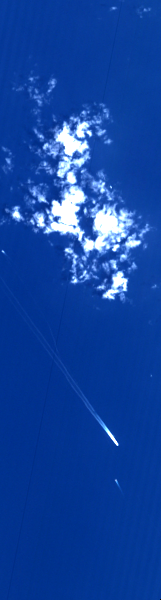
\includegraphics[width=0.15\linewidth]{high_contrast_fragment.png}} &
\fbox{
\includegraphics[width=0.15\linewidth]{mask_pure-water.png}} &
\fbox{
\includegraphics[width=0.15\linewidth]{mask_clouds-tight.png}} &
\fbox{
\includegraphics[width=0.15\linewidth]{mask_wake-tight.png}} \\
Original image & ``pure-water'' & ``clouds-tight'' & ``wake-tight''
\end{tabular}
\end{center}
\caption{Masks used to define sets of pixels for spectral studies. \label{masks}}
\end{figure}

Figure~\ref{masks} shows the three masks I used the most.  The
``pure-water'' mask avoids the wake of the ship, a possible second
ship, and an image defect.  The ``clouds-tight'' includes the thickest
parts of the clouds, and ``wake-tight'' includes the brightest part of
the ship's wake.  I painted over the original image in a separate
layer so that I could remove the original image before saving.  I
chose to paint in red on a white background, so only the green and
blue channels indicate the threshold (red is always 255, green and
blue are sometimes 255 and sometimes 0).  Here's how I loaded the images into NumPy arrays:
\begin{python}
import numpy, PIL
masks = {}
for name in ["cloud-shadow", "pure-water", "image-defect",
            "clouds-loose", "clouds-tight", "wake-loose", "wake-tight"]:
    picture = PIL.Image.open(open("mask_%s.png" % name))
    masks[name] = (numpy.array(picture)[:,:,1] < 128)
\end{python}
Since these masks were made from the {\tt [2200:2800,197:358,:]} image,
it can only be applied to images that have been sliced like that.

\begin{figure}[!b]
\begin{center}
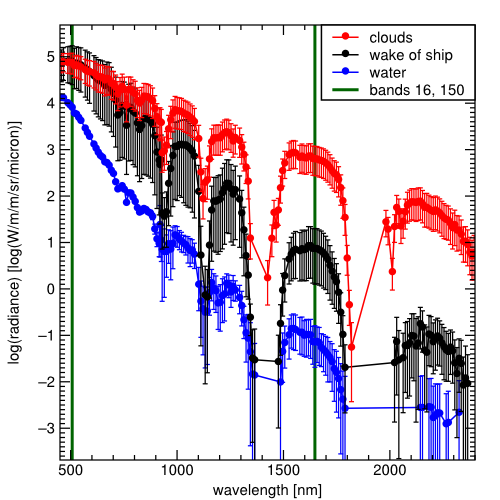
\includegraphics[width=0.75\linewidth]{plots_threespectra.png}
\end{center}
\caption{Spectra of water, clouds, and the wake of the ship.  Bands
  16 and 150 are used in the next section.  Error bars indicate the
  standard deviation of each band over all matching pixels (and {\it
    not} the uncertainty in the mean: see the correlation from band to
  band). \label{plots_threespectra}}
\end{figure}

Now each {\tt masks[name]} is an array of booleans and it can be used
to select pixels from an image using {\tt picture[masks[name]]} where {\tt
  picture} is a $600 \times 161 \times N_{\mbox{\scriptsize bands}}$
array and the result is a $N_{\mbox{\scriptsize selected}} \times
N_{\mbox{\scriptsize bands}}$ array.  I applied this to all the bands
to produce Fig.~\ref{plots_threespectra}.

The first thing we learn from this plot is that the wake of the ship
and the clouds are not the same: they're both much brighter than flat
water, but the clouds have a softer spectrum than the wake.  The
slope of log(radiance) versus wavelength is steepest (bluest) for flat
water, less steep for the ship's wake, and the least steep (reddest)
for clouds.

I think this is extraordinary: we're finding differences among the
spectra of liquid water, liquid water, and liquid water!  The slope
must have something to do with the average size of water droplets,
since that's the only difference I can think of between flat water
(pretty much one big surface), the ship's wake (foam kicked up by the
bow of the ship), and clouds (a diffuse aerosol of microscopic
droplets).  Perhaps each distribution of droplet sizes causes a
different fraction of the sun's light to specular-reflect into the
camera.  The flat sea only specular-reflects at one angle, probably
different from the camera's position, but spherical droplets would
specular-reflect some fraction into the camera just from geometry.

\begin{figure}
\begin{center}
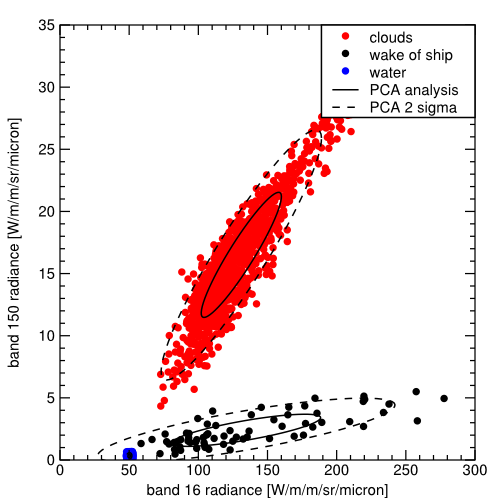
\includegraphics[width=0.75\linewidth]{plots_justtwobands.png}
\end{center}
\caption{Distributions of band 16 and band 150 radiance in for clouds,
  the ship's wake, and water.  Each point in this plot corresponds to
  a pixel in the image. \label{plots_justtwobands}}
\end{figure}

With only two bands, 16 (cannonical blue) and 150 (near infrared), we
can already do some classification.  I made
Fig.~\ref{plots_justtwobands} by loading two raw TIFFs and making
scatter plots in Cassius:

\begin{python}
from cassius import *
from osgeo import gdal, gdalconst

# You would get this from the serialized image.
image016 = gdal.Open(glob.glob(inputDir + "/*_B%03d_L1T.TIF" % 16)[0],
                     gdalconst.GA_ReadOnly)
image150 = gdal.Open(glob.glob(inputDir + "/*_B%03d_L1T.TIF" % %150)[0],
                     gdalconst.GA_ReadOnly)
image016 = image016.GetRasterBand(1).ReadAsArray()[2200:2800,197:358] / 40.
image150 = image150.GetRasterBand(1).ReadAsArray()[2200:2800,197:358] / 80.

water_x, water_y = image016[masks["pure-water"]], \
                   image150[masks["pure-water"]]
wake_x, wake_y = image016[masks["wake-tight"]], \
                 image150[masks["wake-tight"]]
clouds_x, clouds_y = image016[masks["clouds-tight"]], \
                     image150[masks["clouds-tight"]]

waterplot = Scatter(x=water_x, y=water_y, limit=1000, markercolor="blue")
wakeplot = Scatter(x=wake_x, y=wake_y, limit=1000, markercolor="black")
cloudsplot = Scatter(x=clouds_x, y=clouds_y, limit=1000, markercolor="red")

view(Overlay(waterplot, wakeplot, cloudsplot))
\end{python}

Flat water occupies a small spot in at (50, 3) because it is mostly
uniform in these two bands.  Clouds vary in brightness because some
pixels correspond to the tops of clouds, some to their sides, and they vary in
thickness.  However, the brightness in the two bands are strongly
correlated because cloud-material has a consistent spectrum.  The same
can be said for the ship's wake, but with a different slope because of
the different spectral shape.

As described in the first note ({\tt optimized\_color.pdf}), I think
we can describe the spectra of groups of pixels using a Principal
Component Analysis (PCA) of their distribution in a multidimensional
space, where each dimension corresponds to a spectral band.  As you
can already see in Fig.~\ref{plots_justtwobands}, the correlations
among bands is important.  As a first test, I did a simple PCA of these two
bands using a function from Cassius (wraps the NumPy function):
\begin{python}
from cassius import *
origin, xscale, xbasis, yscale, ybasis =
        principleComponents(numpy.array(zip(water_x, water_y)))
\end{python}
The {\tt origin} is the mean of the distribution, {\tt xscale} and
{\tt yscale} are the square roots of the largest two eigenvalues ({\it
  x} is the largest), and {\tt xbasis}, {\tt ybasis} are two-component
eigenvectors.  You can make error ellipses like the ones in
Fig.~\ref{plots_justtwobands} with this:
\begin{python}
waterellipse = Scatter(
    x=[origin[0] + xscale*xbasis[0]*cos(t) + yscale*ybasis[0]*sin(t)
              for t in numpy.arange(0., 2.*pi + 0.1, 0.1)],
    y=[origin[1] + xscale*xbasis[1]*cos(t) + yscale*ybasis[1]*sin(t)
              for t in numpy.arange(0., 2.*pi + 0.1, 0.1)],
    connector="unsorted", marker=None)
\end{python}
(A parametric curve is a scatter plot with no markers and with lines
connecting the points.)

\section{More than two spectral bands}

\begin{figure}[!b]
\begin{center}
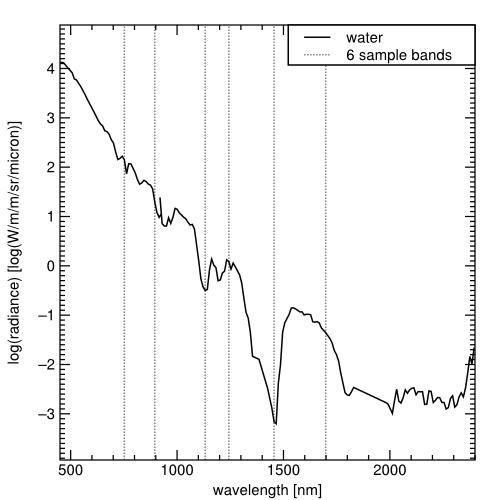
\includegraphics[width=0.45\linewidth]{plot_water_samplebands.png}
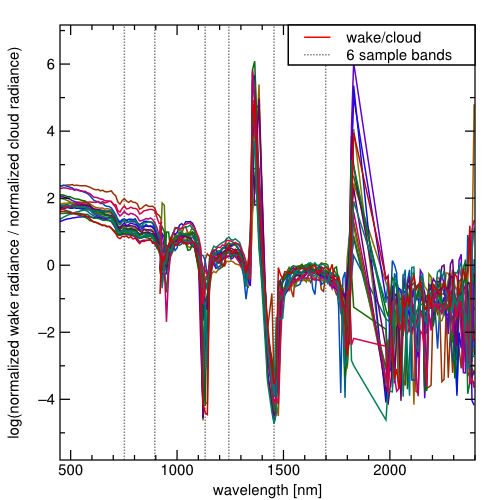
\includegraphics[width=0.45\linewidth]{plot_wakes_clouds_samplebands.png}

\includegraphics[width=0.45\linewidth]{plot_wake_samplebands.png}
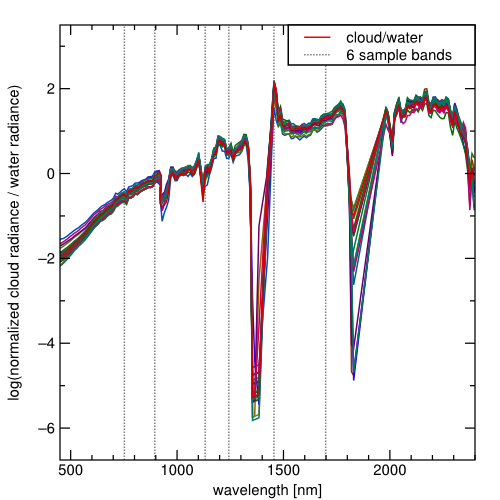
\includegraphics[width=0.45\linewidth]{plot_cloud_samplebands.png}
\end{center}
\caption{Spectral bands chosen for this study, overlaid on (top-left) the
  average water spectrum, (top-right) normalized wake pixels divided
  by cloud (one line-color per pixel, 20 pixels sampled),
  (bottom-left) same for the ratio of wake over water, (bottom-right)
  same for the ratio of clouds over water.  Wake colors vary more
  than cloud colors. \label{plot_water_samplebands}}
\end{figure}

Next, I decided to try something more realistic: more than two bands,
but not (yet?) all the bands.  I chose six bands with roughly maximal
differences between water, wake, and clouds: 40 (752.39 nm), 54
(895.372 nm), 99 (1132.2 nm), 110 (1243.41 nm), 131 (1455.72 nm), and
155 (1698.36 nm).  The plots in Fig.~\ref{plot_water_samplebands} show
the motivation for these choices.

A six-dimensional space is still small enough to visualize.
Figure~\ref{plot_6x6grid} shows the distribution of cloud, wake, and
water radiances in each pair of the six spectral bands.  Much like
Fig.~\ref{plots_justtwobands}, these plots show that radiances in
different bands are highly correlated.  That is, within each category,
the color is roughly constant but the brightness varies.
Figure~\ref{plot_log6x6grid} shows the same thing in log-log scale.

\begin{figure}[p]
\begin{center}
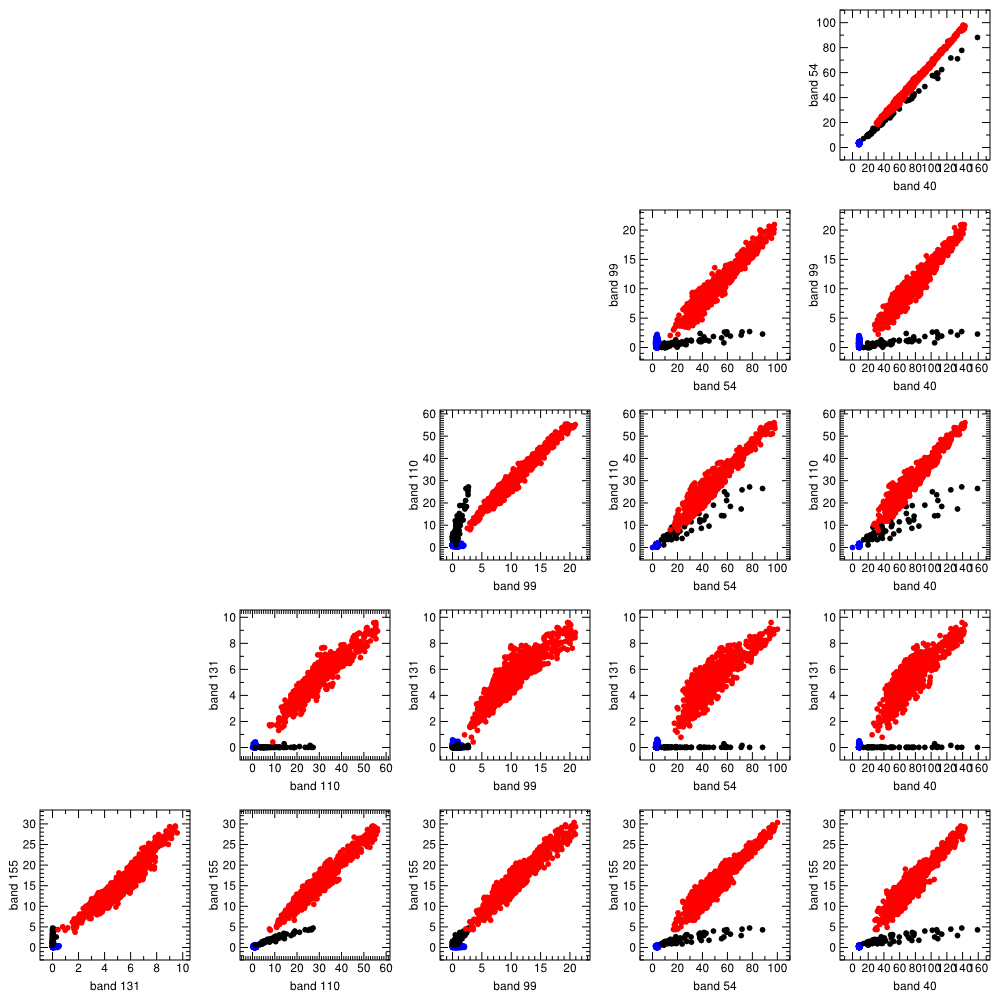
\includegraphics[width=\linewidth]{plot_6x6grid.png}
\end{center}
\caption{Cloud (red), wake (black), and water (blue) radiances in
  each of the six sample bands.  Every pair of distinct bands is
  plotted in a separate window, showing how the distributions overlap
  in all faces of the 6-D hypercube.  White crosses are the medians
  of each distribution. \label{plot_6x6grid}}
\end{figure}

\begin{figure}[p]
\begin{center}
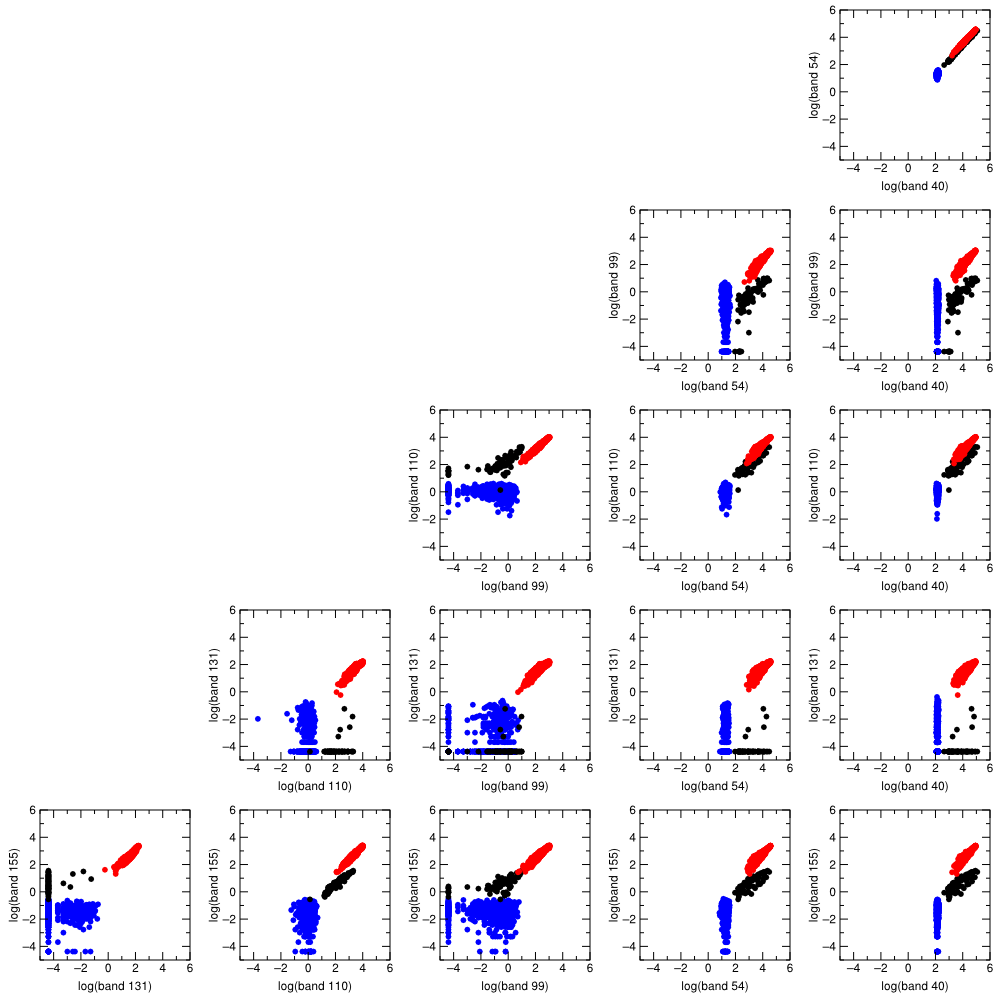
\includegraphics[width=\linewidth]{plot_log6x6grid.png}
\end{center}
\caption{Same as Fig.~\ref{plot_6x6grid} (cloud is red, wake is black,
  and water is blue), but all radiances are shown in log scale,
  providing more detail on the water
  distribution. \label{plot_log6x6grid}}
\end{figure}

Most importantly for identifying ships, the three distributions do not
completely overlap.  We want to manipulate the data to maximize the
separation between ship wakes and everything else, so that ships show
up as bright spots in the images and everything else is dim or
invisible.  The algorithms that take advantage of spatial information
(for example, a bow-wave ``V'' finder) could then start with a high ratio
of signal to background.

First, let's translate the distributions so that water is centered on
zero (it is already near zero).  It is as easy to find medians as it
is to find means, so I use that to avoid dependence on tails.  With
{\tt images} as my {\it height:width:bands} array with six bands,
\begin{python}
import numpy
watercenter = numpy.median(images[masks["pure-water"]], axis=0)
wakecenter = numpy.median(images[masks["wake-tight"]], axis=0)
cloudscenter = numpy.median(images[masks["clouds-tight"]], axis=0)
\end{python}
The results are 1-D, six-element vectors (plotted as white crosses in Fig.~\ref{plot_6x6grid}).

Next, let's remove the clouds.  The vector {\tt cloudscenter -
  watercenter} points from the center of the water distribution
to the center of the cloud distribution: I'd like to construct a
projection operator that projects along this axis (the null space)
onto a plane at the origin, perpendicular to this axis (the range).
Figure~\ref{plot_6x6grid_cloudsremoved} shows the distributions after
this projection: by construction, water and clouds are centered at
zero but the ship's wake is not.  If we declare zero to be black and
distance away from zero to be grey to white, the sea and the clouds
would both be black and the ship's wake would be grey to white.

\begin{figure}[p]
\begin{center}
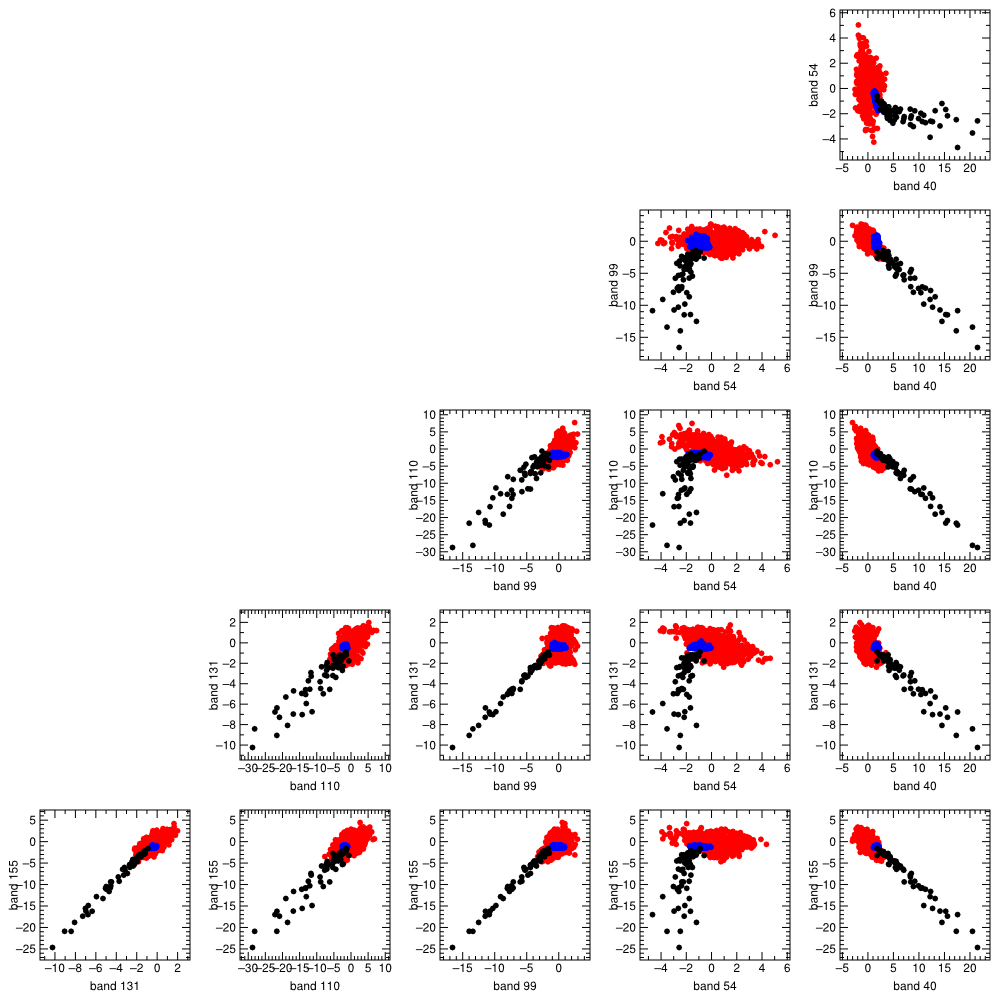
\includegraphics[width=\linewidth]{plot_6x6grid_cloudsremoved.png}
\end{center}
\caption{Same as Fig.~\ref{plot_6x6grid} (cloud is red, wake is black,
  and water is blue), but after translating the origin to the median
  of water and projecting away the axis pointing from the median of
  water through the median of clouds.  Water and clouds are
  centered on zero by construction; wake is maximally separated from both.
 \label{plot_6x6grid_cloudsremoved}}
\end{figure}

The projection operator is constructed in two steps.  First we find an
orthonormal basis in which one of the basis vectors points in the
direction of {\tt cloudscenter - watercenter}.  This basis is not
unique, but the choice of the other five basis vectors is not
important.  Most linear algebra packages provide a QR factorization
for producing an orthonormal basis, but they use algorithms that don't
guarantee that the first one points along a given axis (for more
numerical stability).  The following implementation of a simple
Gram-Schmidt process guarantees that the first output ({\tt us[0]}) is
parallel to the first input ({\tt vs[0]}).
\begin{python}
import numpy
def gramSchmidt(vs):
    us = []
    for i, v in enumerate(vs):
        u = numpy.array(v)
        for j in xrange(i):
            u -= us[j].dot(v) * us[j]
        u /= numpy.linalg.norm(u)
        us.append(u)
    return us
\end{python}

Since we don't care about the distribution of the other five basis
vectors ({\tt us[1:6]}), we can feed it a random set of input
vectors.  (The unit-normal distribution from {\tt numpy.random.randn}
minimizes numerical instability, which is a problem for the
Gram-Schmidt algorithm.)
\begin{python}
basis = gramSchmidt([cloudscenter - watercenter] +
                        zip(*numpy.random.randn(6, 5)))
\end{python}
Now {\tt basis} is a list of six 6-D unit vectors, the first is
parallel to {\tt cloudscenter - watercenter} and the rest are
perpendicular to {\tt cloudscenter - watercenter} and each other.

The second step is to build the projection operator.  Ideally, this
should be a vectorized NumPy procedure so that it can be applied to a
huge dataset (such as a large image) without any Python calls in the
loop.  I was lazy and just wrote a lambda expression, so it's a lot
slower than it needs to be.  If we scale this up, I should rethink the
implementation.
\begin{python}
projection = lambda x: sum([w * w.dot(x) for w in basis[1:]])
\end{python}
In symbols, this is
\begin{equation}
\mbox{\tt projection}_W(\vec{x}) = \sum_{i=1}^5 (\vec{x} \cdot \vec{w}_i) \, \vec{w}_i
\end{equation}
where $\vec{w}_i \in W$ is the space orthogonal to {\tt basis[0]} and
$\vec{x}$ is any vector.

To see what it looks like to remove clouds, we can apply the
projection operator to an image, band 40 (closest to visible light in
our {\tt sampleBands}).

\begin{python}
import numpy, PIL

for i in xrange(len(sampleBands)):
    image[:,:,i] -= watercenter[i]    # center on water

# Linearize height and width, apply projection, then restore the structure
projimage = numpy.reshape(image,
                          (image.shape[0]*image.shape[1], image.shape[2]))
projimage = numpy.array(map(projection, projimage))
projimage = numpy.reshape(projimage,
                          (image.shape[0], image.shape[1], image.shape[2]))

band = projimage[:,:,sampleBands.index(40)]  # select band 40

minvalue = 1.   # cuts out clouds and water, both centered at zero
maxvalue = 10.  # rough maximum for this band
band = numpy.array(numpy.maximum(numpy.minimum((band - minvalue) /
                   (maxvalue - minvalue) * 255., 255), 0), dtype=numpy.uint8)

image = numpy.dstack((band, band, band))
image = PIL.Image.fromarray(image)
image.save("/var/www/quick-look/tmp.png", "PNG", options="optimized")
\end{python}

The resulting image is shown in Fig.~\ref{cloud_removal}.

\begin{figure}[!b]
\begin{center}
\begin{tabular}{c c}
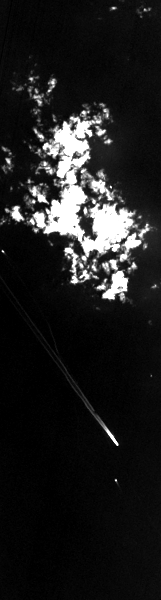
\includegraphics[width=0.28\linewidth]{cloud_removal_before.png} &
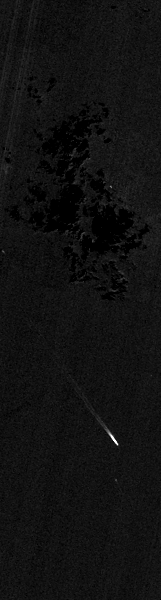
\includegraphics[width=0.28\linewidth]{cloud_removal_after.png} \\
Before & After
\end{tabular}
\end{center}
\caption{The image in band 40, before and after cloud-removal.  The
  cloud and the water become dark without sacrificing too much
  intensity in the ship's wake.  The {\tt minvalue} threshold set by
  hand in the code controls how much of the cloud the human eye
  detects.  \label{cloud_removal}}
\end{figure}

\section{Background likelihood}

Now that we have a way of making the clouds look like the background
(flat water), we want to use the six-dimensional information to color
the pixels in a way that maximizes the difference between signal and
background.  The example shown in Fig.~\ref{cloud_removal} uses only
one band (40) and a threshold that was set by hand ({\tt minvalue}).
I'd like to find an automated solution to get better results with less
arbitraryness, but I haven't yet found one that outperforms
Fig.~\ref{cloud_removal}.

The idea described in {\tt optimized\_color.pdf} is to
treat the background distribution as a Gaussian blob with
correlations.  That is, do a PCA analysis on everything (which is
mostly background) to get the parameters of a best-fit Gaussian error
ellipse.  I take this as the likelihood distribution and color pixels
by their unlikelihood.  By construction, the ship's wake pixels
contain the least likely combination of the six bands and hence should
stand out.

The PCA analysis is (1) find the covariance of the set of 6-D vectors,
one for each pixel in the image, (2) find the eigenvalues and
eigenvectors of that covariance matrix, and (3) remove the smallest
one.  Step (3) is only needed because our data is effectively
five-dimensional, now that we've projected away the clouds.  It shows
up in the eigenvalues as a nearly-zero eigenvalue ({\tt 1e-16},
machine precision).  Since we no longer have any information along
this direction (we threw it all away), this axis of the error ellipse
should be infinite, so I set it to a large number ({\tt 1e10}, but
since our data has been projected, any number larger than {\tt 1e-16}
would do).

The eigenvalues and eigenvectors together define a matrix that
transforms our dataset to a spherically symmetric unit Gaussian (plus
any unmodeled tails).  The likelihood in that space is
$\exp(-|\vec{x}|^2)$, so we get the likelihood in our space by untransforming.

\begin{python}
from math import *
import numpy

# Linearize height and width and apply projection
projimage = numpy.array(map(projection,
    numpy.reshape(image, (image.shape[0]*image.shape[1], image.shape[2]))))

# Perform the PCA analysis.
eigenvalues, eigenvectors = numpy.linalg.eig(numpy.cov(projimage.T))
smallestIndex = numpy.argsort(eigenvalues)[0]
eigenvalues[smallestIndex] = 1e10

# Define a likelihood function using the eigenbasis.
def likelihood(p0, p1, p2, p3, p4, p5):
    return exp(-sum(numpy.square(numpy.array(
        numpy.matrix([[p0, p1, p2, p3, p4, p5]]) * eigenvectors).flatten())
        / eigenvalues))
\end{python}

Figure~\ref{plot_6x6grid_likelihood} shows slices through the
likelihood function overlaid by wake pixels.

\begin{figure}
\begin{center}
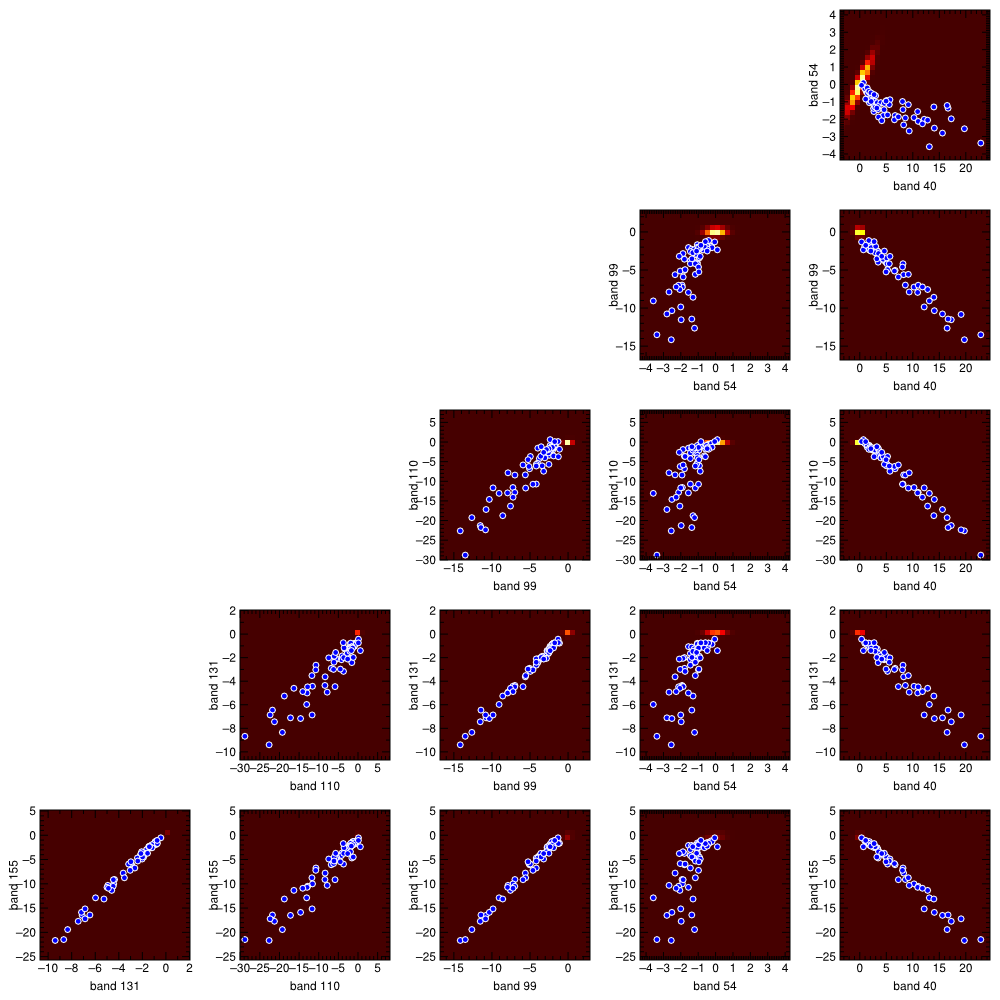
\includegraphics[width=\linewidth]{plot_6x6grid_likelihood.png}
\end{center}
\caption{The color field is the likelihood function, sliced through
  each pair of bands.  Yellow is maximum likelihood, magenta is
  minimum.  The blue points are the ship's wake data, which extend
  beyond the first few sigma in likelihood.
 \label{plot_6x6grid_likelihood}}
\end{figure}

\pagebreak
To turn the likelihood values into pixel colors, we need to transform
the likelihood's very broad interval to a manageable interval like (0,
1).  Note that the negative log-likelihood,
\begin{python}
def loglikelihood(p0, p1, p2, p3, p4, p5):
    return sum(numpy.square(numpy.array(
        numpy.matrix([[p0, p1, p2, p3, p4, p5]]) * eigenvectors).flatten())
        / eigenvalues)
\end{python}
is just a $\chi^2$.  (The usual formula for $\chi^2$ is $\sum_i^N (y_i
- y(x_i))^2/{\sigma_i}^2$, but here $y(x_i) = 0$ and $\sigma_i = 1$
because we've transformed to the space in which the model is a unit
Gaussian.)  Therefore, we can use a $\chi^2$ cumulative distribution
function to map {\tt loglikelihood} to (0, 1).  SciPy provides such a
function:
\begin{python}
from scipy.stats import chi2 as chi2prob
def normalize(x):
    return chi2prob.cdf(x, 5)   # 5 d.o.f
\end{python}

Once the distribution is in the unit interval, we map to (0, 255) the
normal way (see code fragments involving {\tt minvalue} and {\tt maxvalue}).

\begin{figure}[p]
\begin{center}
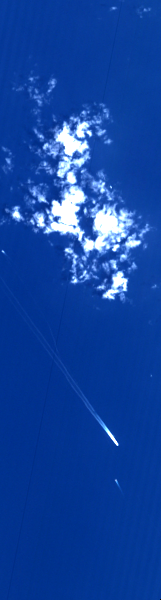
\includegraphics[width=0.28\linewidth]{high_contrast_fragment.png}
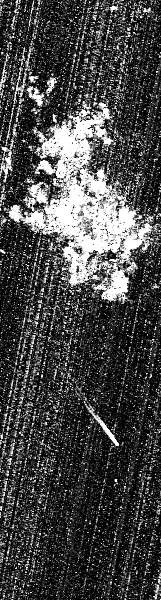
\includegraphics[width=0.28\linewidth]{likelihood_image.png}
\end{center}
\caption{Original RGB image (left) and image produced by a Gaussian
  likelihood (right).  The ship was easier to see before we did
  anything! \label{likelihood_image}}
\end{figure}

The result in Fig.~\ref{likelihood_image} is somewhat disappointing:
this method found the ship's wake, but it also brought out image
defects that were only faintly visible in the normal view and it
hasn't suppressed the cloud.  My conclusion is that defects are
non-Gaussian tails and the cloud is non-Gaussian as well.  Even if I
cheat and apply the PCA algorithm to the cloud pixels only, the edges
of the cloud are still visible because the distribution just isn't
round.

We can suppress the tails by exaggerating the unlikelihood function.
For instance, once the values are mapped to the unit interval, we can
apply {\tt numpy.power(unitIntervalData, 10)} to bring out highly
unlikely features at the expense of less unlikely features.  The
result is a dot at the ship's wake with no image defects or clouds,
but the dot loses most of its spatial distribution.  The bow of the
wake is at an extreme of the unlikelihood, but not the two separating
waves.

\section{Another idea: Na\"ive Bayes}

Since the tails of the distribution are important, I tried a Na\"ive
Bayes approach.  I originally didn't consider Na\"ive Bayes because
correlations among parameters are so important.  To add a simple handling of
correlations, I first transformed by the matrix of eigenvectors from
the PCA, then applied Na\"ive Bayes in the eigenspace.  That way, the
marginal distributions would at least be aligned with the shape of the
blob.

After subtracting the water and projecting away the clouds, I
transformed the distributions like this:
\begin{python}
def transformation((p0, p1, p2, p3, p4, p5)):
    return numpy.array(numpy.matrix([[p0, p1, p2, p3, p4, p5]])
        * eigenvectors).flatten() / numpy.sqrt(eigenvalues)
projimage_trans = numpy.array(map(transformation, projimage))
projwake_trans = numpy.array(map(transformation, projwake))
\end{python}

I then built a likelihood on the transformed distributions using
Cassius histograms (just because they were readily available).
\begin{python}
from math import *
from cassius import *

projimage_0 = Histogram(100, -50., 50., data=projimage_trans[:,0])
projimage_1 = Histogram(100, -20., 20., data=projimage_trans[:,1])
projimage_2 = Histogram(100, -20., 20., data=projimage_trans[:,2])
projimage_3 = Histogram(100, -20., 20., data=projimage_trans[:,3])
projimage_4 = Histogram(100, -1., 1., data=projimage_trans[:,4])
projimage_5 = Histogram(100, -10., 10., data=projimage_trans[:,5])

wake_0 = Histogram(100, -50., 50., data=projwake_trans[:,0])
wake_1 = Histogram(100, -20., 20., data=projwake_trans[:,1])
wake_2 = Histogram(100, -20., 20., data=projwake_trans[:,2])
wake_3 = Histogram(100, -20., 20., data=projwake_trans[:,3])
wake_4 = Histogram(100, -1., 1., data=projwake_trans[:,4])
wake_5 = Histogram(100, -10., 10., data=projwake_trans[:,5])

def loglikelihood(x):
    x = transformation(x)
    denom_loglikelihood = 0.
    numer_loglikelihood = 0.
    for i, (denomhist, numerhist) in enumerate([
            (projimage_0, wake_0), (projimage_1, wake_1), (projimage_2, wake_2),
            (projimage_3, wake_3), (projimage_5, wake_5)]):
            # 4 is excluded because that's the cloud removal eigenvector
        index = denomhist.index(x[i])
        if index is None:
            denom_loglikelihood += log(1. / denomhist.entries)
            numer_loglikelihood += log(1. / numerhist.entries)
        else:
            denomvalue = denomhist.values[index] + 1e-5
            numervalue = numerhist.values[index] + 1e-5
            denom_loglikelihood += log(denomvalue / denomhist.entries)
            numer_loglikelihood += log(numervalue / numerhist.entries)
    return numer_loglikelihood / denom_loglikelihood
    # Last minute note: shouldn't the division in the last line be subtraction???
\end{python}

These histograms are shown in Fig.~\ref{plot_naivebayes_with_pca}.

\begin{figure}
\begin{center}
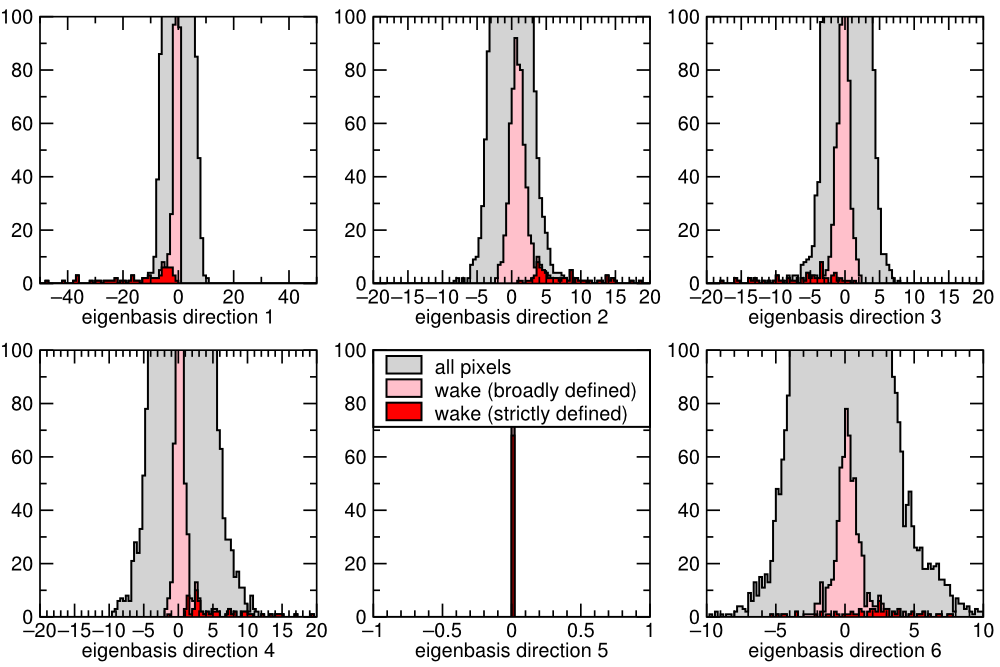
\includegraphics[width=\linewidth]{plot_naivebayes_with_pca.png}
\end{center}
\caption{Distributions used to define likelihood for the Na\"ive Bayes analysis.  Strictly defined wake (red) is the definition I've been using in most of this document; loosely defined wake (pink) is a superset including a few more of the surrounding pixels (highly contaminated by water spectra).  Eigenbasis direction 5 is the axis that was projected to remove clouds (skipped in the analysis). \label{plot_naivebayes_with_pca}}
\end{figure}

\begin{figure}
\begin{center}
\begin{tabular}{c c c}
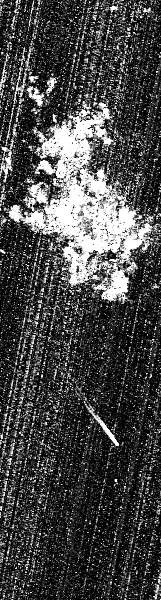
\includegraphics[width=0.28\linewidth]{likelihood_image.png} &
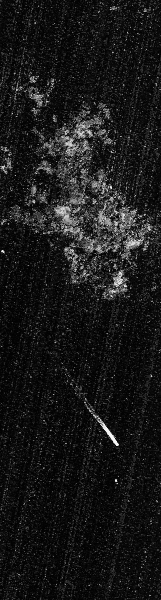
\includegraphics[width=0.28\linewidth]{likelihood_naivebayes_image.png} &

\includegraphics[width=0.28\linewidth]{likelihood_naivebayes_power10_image.png} \\
Gaussian likelihood & Na\"ive Bayes likelihood & Raised to the 10$^{\mbox{\scriptsize th}}$ power
\end{tabular}
\end{center}
\caption{Final comparison of images: the Gaussian likelihood (left) re-shown from Fig.~\ref{likelihood_image}, Na\"ive Bayes (middle) is the product of this analysis, and raised to the 10$^{\mbox{\scriptsize th}}$ power applies {\tt numpy.power(unitIntervalData, 10)} to bring out highly unlikely features. \label{likelihood_naivebayes_image}}
\end{figure}

\section{Applying the algorithm to whole images}

Figure~\ref{whole_image_allthree} shows what the algorithm looks like
when applied to whole images, rather than just the training sample.
Land features are unlikely in the training data, so they show up as
well as the ships' wakes.  When aligned and overlaid on Google Maps
images, this won't be a problem for a human because the demarcation
between land and sea would be obvious.  For an automatic ship-finder,
the land would be at least as confusing as clouds--- if the spatial
algorithm can handle land, then we might as well leave the clouds in,
too.

In the final images, we can see the ship's wake that we used for training
(just barely), and possibly two more in the third image.

\begin{figure}[!b]
\begin{center}
\includegraphics[width=0.8\linewidth]{whole_image_allthree.png}
\end{center}
\caption{The Na\"ive Bayes raised to the tenth power method, applied to all three Kagoshima Bay images.  The training image is on the left. \label{whole_image_allthree}}
\end{figure}

\section{A much simpler algorithm}

I still don't understand why it's so hard to see the ship's wake in
the fully processed images when wake, cloud, and water distributions
are easily seperable in Fig.~\ref{plots_justtwobands}.  For
comparison, I did a much simpler, cuts-based analysis.
Figure~\ref{plots_simplecut} shows the same data as
Fig.~\ref{plots_justtwobands} with
\begin{python}
cut = (image016 - 2. > (1000. - 2.)/100.*image150)
\end{python}
That is, a line starting 2 units to the right of the origin with slope
100.  This should cleanly separate between clouds and wake.

\begin{figure}
\begin{center}
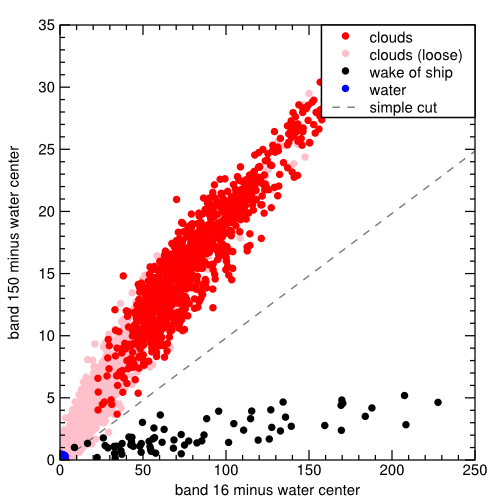
\includegraphics[width=0.75\linewidth]{plots_simplecut.png}
\end{center}
\caption{Clouds (tight and loose), wake, and water distributions with
  a cut in the two-dimensional space of band 16 (cannonical blue) and
  band 150 (near infrared) to separate clouds from wake. \label{plots_simplecut}}
\end{figure}

We then define brightness in the image simply by band 16 (cannonical
blue) to make Fig.~\ref{simplecut_image}.  The wake is bright and the
clouds are suppressed.

\begin{figure}
\begin{center}
\begin{tabular}{c c c}
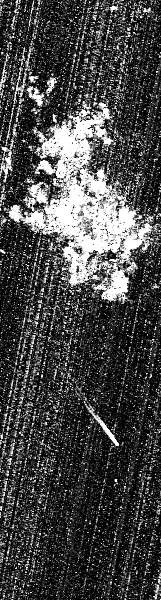
\includegraphics[width=0.28\linewidth]{likelihood_image.png} &
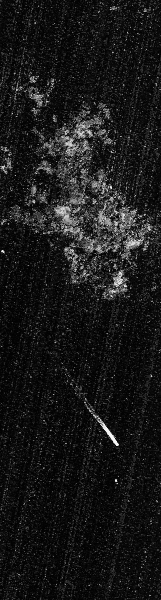
\includegraphics[width=0.28\linewidth]{likelihood_naivebayes_image.png} &
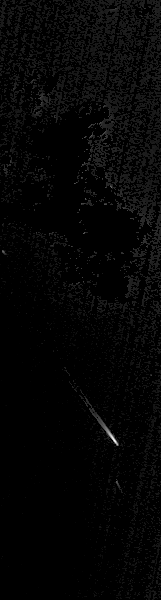
\includegraphics[width=0.28\linewidth]{simplecut_image.png} \\
Gaussian likelihood & Na\"ive Bayes & Simple cut
\end{tabular}
\end{center}
\caption{Final images from the three analyses.  The simple cut in two
  bands does everything we need it to.  But is it overtrained?  Can
  the hand-selected cut values be automated reliably? \label{simplecut_image}}
\end{figure}

\pagebreak
While the simple cut method is much better at identifying the known
ship in the training data, it does worse than Na\"ive Bayes on
different datasets.  (Neither method was re-trained for different
datasets--- Na\"ive Bayes is somehow more stable against changes in conditions.)

\begin{figure}[!b]
\begin{center}
\includegraphics[width=0.8\linewidth]{whole_simplecut_allthree.png}
\end{center}
\caption{The simple cut method, applied to all three Kagoshima Bay
  images.  The training image is on the left.  While this method does
  not highlight the ground, it is too sensitive to changes in
  conditions.  See Fig.~\ref{whole_image_allthree} for a comparison to Na\"ive Bayes. \label{whole_simplecut_allthree}}
\end{figure}

\section{Conclusion}

None of the resulting methods are satisfactory, but hopefully these
code samples will be useful in constructing an optimal method.

Perhaps I've been too focused on eliminating clouds.  Do we need to
eliminate clouds?  None of the methods described here would reveal
whatever is below the clouds--- they just zero out the clouds so that
they're not a source of confusion to a later algorithm in the
workflow.  But ground features on shore would be just as confusing to
an automated algorithm.

Maybe I've been doing the wrong thing by projecting out the clouds as
a linear transformation in radiance.  Maybe it should be in
log(radiance) because absorbtion is multiplicative.

The very last line in my {\tt loglikelihood} function for Na\"ive
Bayes has a division that I think should be a subtraction.

Maybe we could do clustering in spectrum space to find the major
components.  Clusters close to what we expect for water and for clouds
could then be labeled as such and we can define brightness as distance
away from the bad clusters.  (That's equivalent to centering the water
distribution and then projecting out the clouds and calling the origin
the bad cluster center.)

Other ideas???

\end{document}
